\section{Requirements and Preliminaries}
\label{sec:background}

\subsection{Requirements}

Our goal is to establish a bi-directional communication link using visible lights. As the dual-paradigm nature of VLC over the lighting infrastructure entails that the primary function is illumination and the primary usage scenario is communicating with low power mobile devices or sensor nodes, we have the following two basic requirements behind the goal. 

\noindent\emph{\textbf{Requirement 1:}} Establish a low-power, duplex visible light communication link with a battery-free mobile end that harvests light energy from the illumination LED. 

\noindent\emph{\textbf{Requirement 2:}} Impose no constraints on the actual usage. This implies a practical working range in normal indoor situations, ease of use, and that the size of the device should be small for convenience.

To achieve a duplex visible link, one possibility is to use a symmetric design, that is, using an LED on the mobile device or sensor node to actively emit signals, which are picked up by a light sensor on the lighting LED. Unfortunately, to be able to reach a practical working distance (with the light typically installed on the ceiling) costs prohibitively high energy on the mobile device of a credit card size. Being electromagnetic radio in nature, the light energy attenuates quickly as propagation proceeds~\cite{lightwave}.

One way to extend the communication range is to use directional signals, ideally a laser. However, that would require manual alignment between the light source and the mobile device. 

Another possible way towards more affordable power is to leverage the light from the lighting infrastructure, which is usually of high power. This is similar to the design of passive RFID systems where the tag communicates with the reader by reflecting the incoming radio signal. For instance, we may use a \textit{mirror} to reflect the light from the LED back to a light sensor collocated on the LED. However, a mirror makes highly directional reflection. Such a design would also require carefully orienting the mobile device and violate the practicality requirement. 

Inspired by free space laser communication systems~\cite{mrr}, we use a retro-reflector to meet requirement 2. Below we introduce the retro-reflector and present some favorable properties about retro-reflector materials. 



\subsection{Preliminaries}

\begin{figure}[tb]
    \centering
    \subfigure[Corner Cube Illustration]{
        \includegraphics[width=0.45\columnwidth]{../illustrations/retroreflector.eps} 
        \label{fig:cornercube}
    } \hfill
    \subfigure[Bicycle Retro-reflector]{
        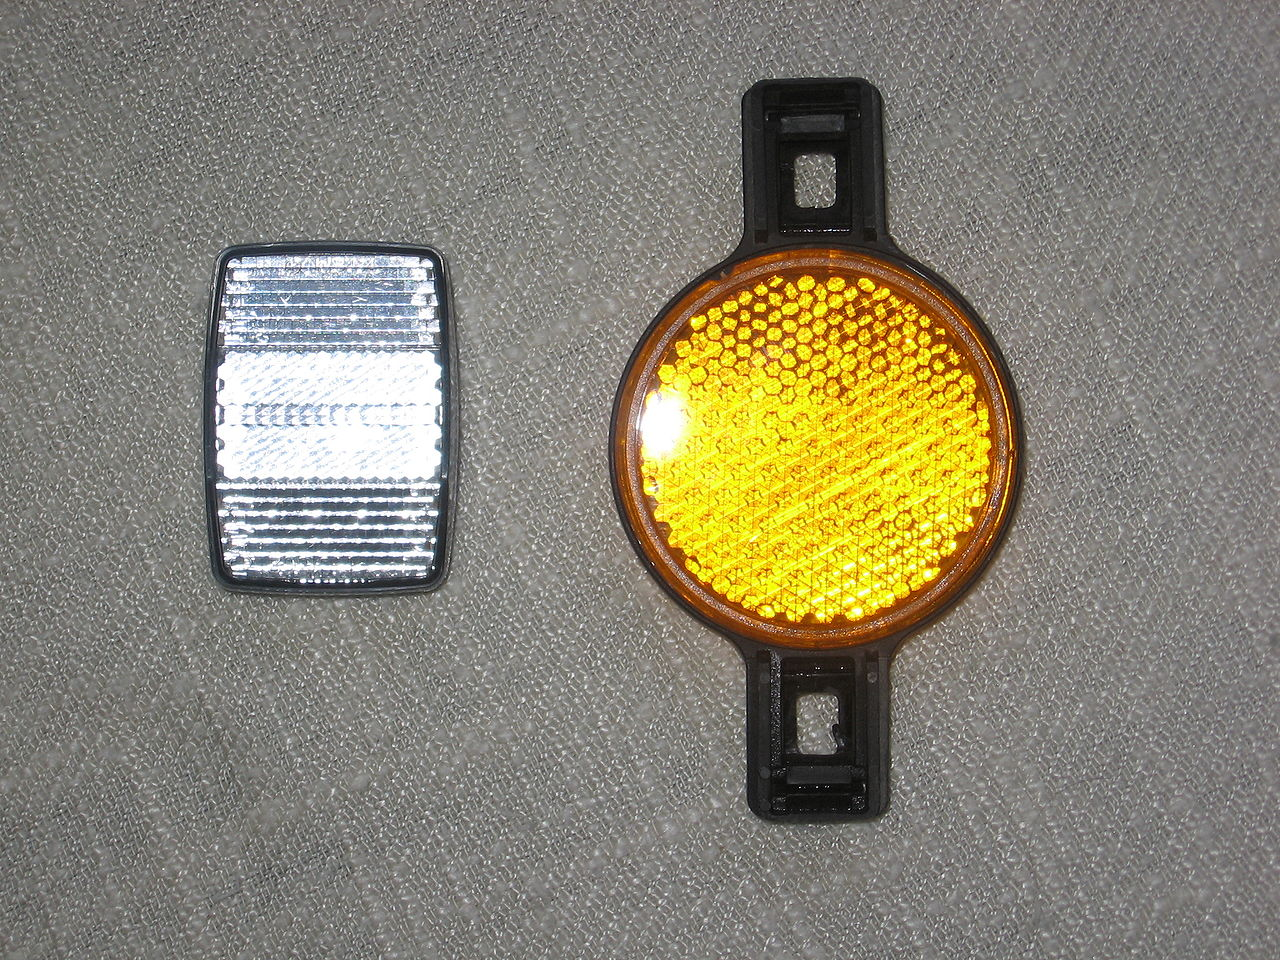
\includegraphics[width=0.45\columnwidth]{1280px-BicycleRetroreflectors.jpg}
        \label{fig:bike-cc}
    } 
     \caption{\label{fig:retro-reflector}Principle of a retro-reflector and sample products.}
%      \vspace{-5mm}
  \end{figure}

\paragraph{Retro-reflector} 
A retro-reflector is a device or surface that, unlike mirrors, reflects light back to its source along the same incoming direction with little scattering~\cite{rr}. 

A retro-reflector can be produced using spherical lens, much like the mechanism of a cat's eye. A more feasible way to obtain retro-reflection is to use a corner reflector, which consists of a set of cubes each with three mutually perpendicular reflective surfaces. The principle of such a retro-reflector is shown in \figref{fig:cornercube}. A large yet relatively thin retroreflector is possible by combining many small corner reflectors, using the standard triangular tiling. Such thin retro-reflectors are widely used on road signs, bicycles, and clothing for safety. \fyi{\figref{fig:bike-cc} shows a flattened retro-reflector seen on bicycles.} \todo{May merge Fig 1 and 2, by removing the current fig 2(d).}


%\begin{figure*}[!th]
%  \begin{center}
%      \subfigure[TX $90\degree$, RX $90\degree$]{
%        \includegraphics[height=0.2\columnwidth]{../illustrations/mrr4.eps}\label{fig:mrr4}
%      } 
%      \hfill
%      \subfigure[TX $45\degree$, RX $45\degree$]{
%        \includegraphics[height=0.2\columnwidth]{../illustrations/mrr1.eps}\label{fig:mrr1}
%      } 
%      \hfill
%      \subfigure[TX $45\degree$, RX $90\degree$]{
%        \includegraphics[height=0.2\columnwidth]{../illustrations/mrr3.eps}\label{fig:mrr3}
%      }
%%      \vspace{-1em}
%      \caption{Optical properties of a retro-reflector fabric, comparing with a white paper and a planar mirror. (a) When the LED is at $90\degree$, and the camera is at $90\degree$, both the retro-reflector and mirror areas are bright. (b) When the LED (TX) is at $45\degree$ arrival of incidence, and the camera (RX) is at $45\degree$, the retro-reflector area (on the right) is bright, the mirror area (in the middle) is dark, and the paper area (on the left) is dark. (c) When the LED is at $45\degree$, and the camera is at $90\degree$, the retro-reflector and the mirror areas are dark, while the paper area is slightly bright due to diffused reflections. \todo{Need to separate the figures without LCD. Make sure the exposure to be the same. Pay attention to the aspect ratio.}}\label{fig:rr-reflection}
%  \end{center}
%%  \vspace{-0.3in}
%\end{figure*}

\iftrue
\begin{figure}[th]
  \begin{center}
      \subfigure[Flash at $90\degree$, Camera at $90\degree$]{
        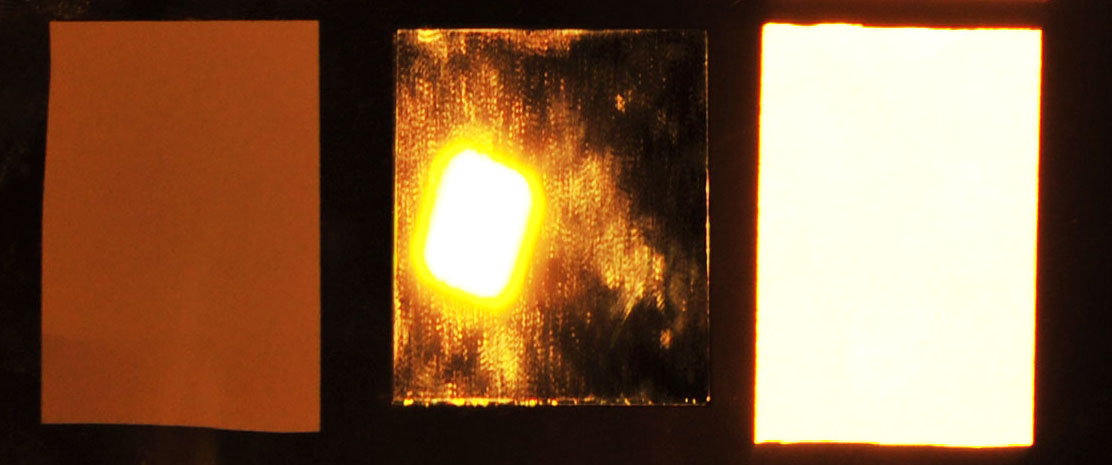
\includegraphics[width=0.46\columnwidth]{tx90-rx90.jpg}\label{fig:mrr4}
      } 
      \hfill
      \subfigure[Flash at $45\degree$, Camera at $90\degree$]{
        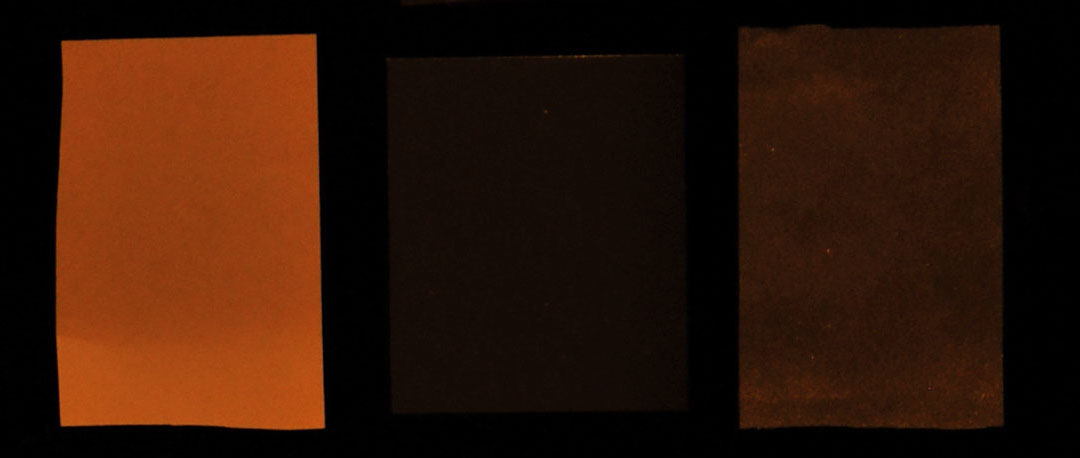
\includegraphics[width=0.45\columnwidth]{tx45-rx90.jpg}\label{fig:mrr3}
      } \\
      \subfigure[Flash at $45\degree$, Camera at $45\degree$]{
        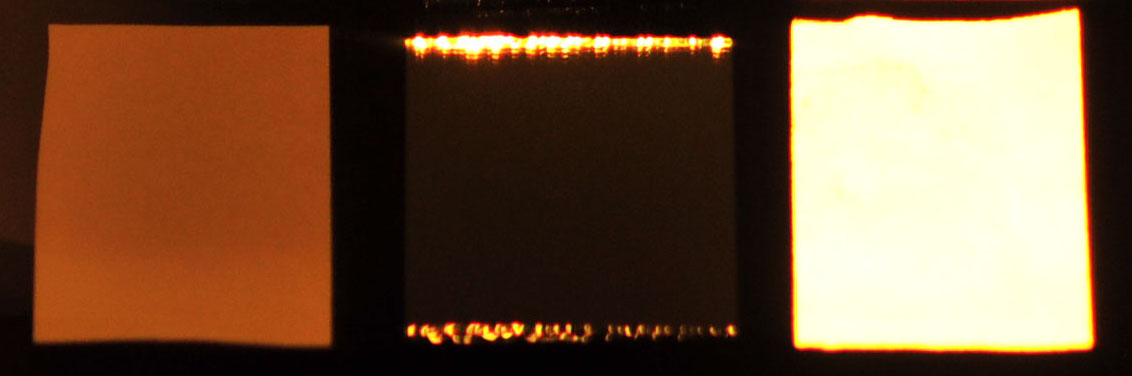
\includegraphics[width=0.45\columnwidth]{tx45-rx45.jpg}\label{fig:mrr1}
      } 
      \hfill \hspace{-1ex}
    \subfigure[Reflection dispersion]{
        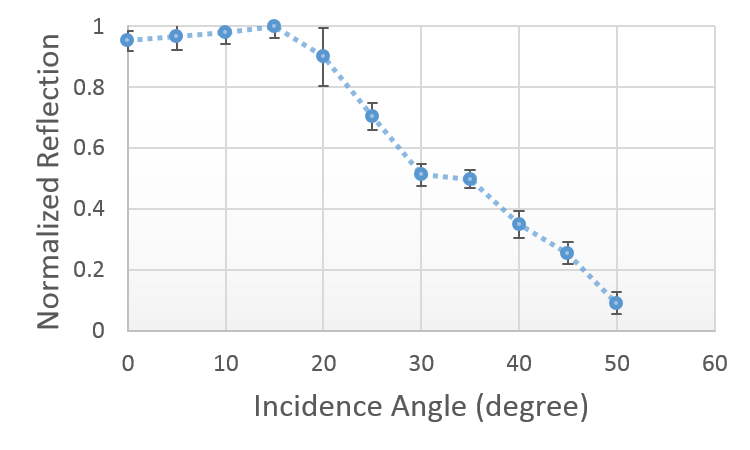
\includegraphics[width=0.5\columnwidth]{rr-angle.png}
        \label{fig:rr-angle}
    } 

%      \vspace{-1em}
      \caption{Optical reflection properties of a retro-reflector fabric (Scotchlite from 3M) (right), compared with a white paper (left) and a planar mirror (middle).}\label{fig:rr-reflection}
  \end{center}
%  \vspace{-0.3in}
\end{figure}
\else
\begin{figure}[!th]
  \begin{center}
    \subfigure[Reflection property]{
        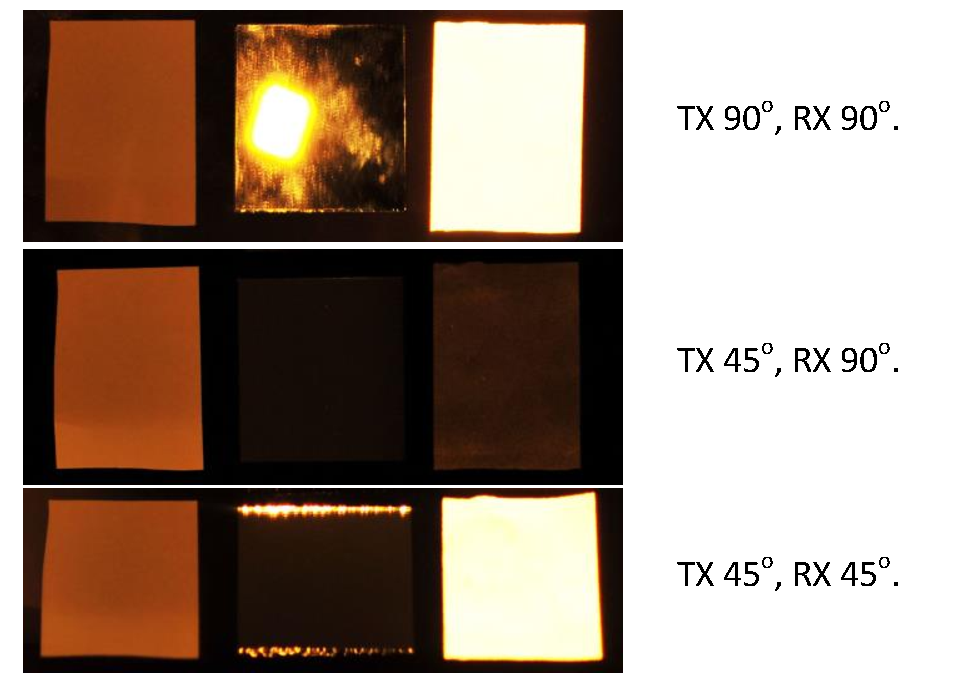
\includegraphics[width=0.9\columnwidth]{RR-property-exp.pdf}
        \label{fig:rr-exp}
    } \\
    \subfigure[Reflection property]{
        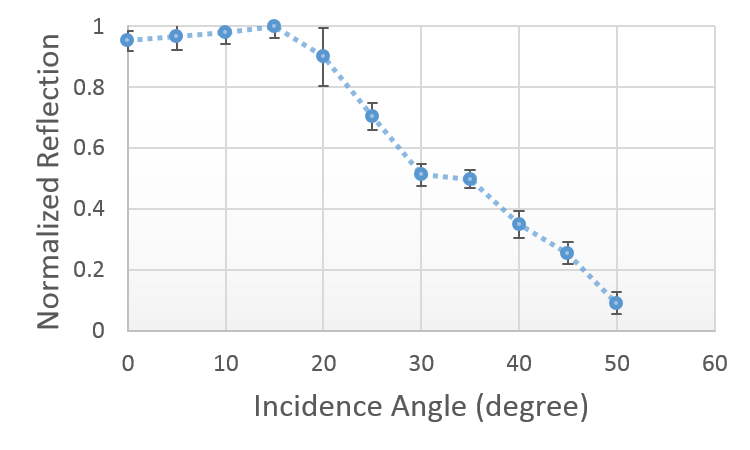
\includegraphics[width=0.7\columnwidth]{rr-angle.png}
        \label{fig:rr-angle}
    } 

%      \vspace{-1em}
      \caption{Optical properties of a retro-reflector fabric, comparing with a white paper and a planar mirror. \todo{Need to separate the figures without LCD. Make sure the exposure to be the same. Pay attention to the aspect ratio.}}\label{fig:rr-reflection}
  \end{center}
%  \vspace{-0.3in}
\end{figure}
\fi


%      \vspace{-5mm}

We conduct experiments to measure the reflecting properties of our retro-reflector fabric (Scotchlite from 3M~\cite{rrsheet}). We compare it against a plain white paper which features diffusing reflection and a planar mirror that does mirror reflection. We place the three materials side by side and let the light source (a flash light) emit light at different angles while retaining the same distance to the materials. We use a camera to capture reflected light. \figref{fig:rr-reflection} shows the resulting images from experiments conducted in a dark chamber. In the figures, we can see that the retro-reflector fabric is bright as long as the light source and the camera are along the same direction, be it $45\degree$ or $90\degree$, whereas the mirror is bright only when both the camera and the flash are at $90\degree$. In case (c), the images of the mirror and the retro-reflector are dark. On the contrary, the white paper is always slightly turned on despite the flash and camera positions because of the diffusion.  
%\todo{(a) When the LED is at $90\degree$, and the camera is at $90\degree$, both the retro-reflector and mirror areas are bright. (b) When the LED is at $45\degree$, and the camera is at $90\degree$, the retro-reflector and the mirror areas are dark, while the paper area is slightly bright due to diffused reflections. (c) When the LED (TX) is at $45\degree$ arrival of incidence, and the camera (RX) is at $45\degree$, the retro-reflector area (on the right) is bright, the mirror area (in the middle) is dark, and the paper area (on the left) is dark.} 
We notice that the brightness of the retro-reflector tends to be weaker than that of the mirror but more uniform. This is because the retro-reflector fabric is not perfect. \fyi{Further measurements show that such dispersion is severed when the incidence angle is over $\pm20\degree$, as shown in \figref{fig:rr-angle}.}

%\paragraph{Modulating Retro-reflector}
%Modulating retro-reflector (MRR)~\cite{mrr} consists of a retro-reflector and a modulator for optical communications. An MRR operates as a passive sources which transmits bits by varying the intensity of the reflected light beam. MRR is widely used in free space communication where the other side is a laser. Existing MRR systems~\cite{expensive,expensive2} is usually of a large size, and modulation is commonly achieved with a high-end electroabsorption modulator altering the absorption spectrum by applying an electric field. Consequently, such setting is ill-suited for our scenarios which require a low-cost solution.

The ability to bounce back light from any incidence angle leads to a favorable property of a retro-reflector: when the light source emits omni-directional lights, the retro-reflector will concentrate the lights as it reflects them. This is illustrated in \figref{fig:retro1}. From experiments, we empirically found that the concentrated energy is directly proportional to the size of the retro-reflector fabric, as shown in \figref{fig:retro2}. This property enables us to achieve higher reflected signal strength by using larger retro-reflector.
\begin{figure}[!th]
  \begin{center}
      \subfigure[Energy Concentration]{
        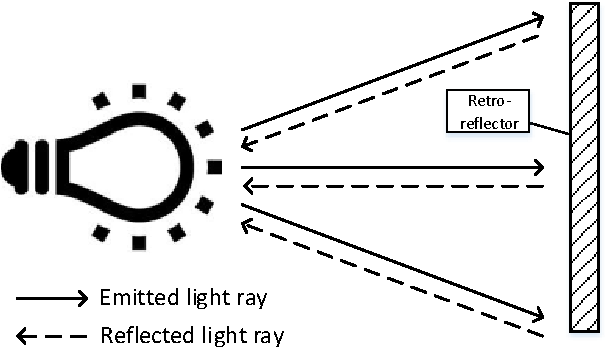
\includegraphics[width=0.46\columnwidth]{retro-reflector.pdf}\label{fig:retro1}
      } 
      \hfill
      \subfigure[Reflected Energy vs. Area]{
        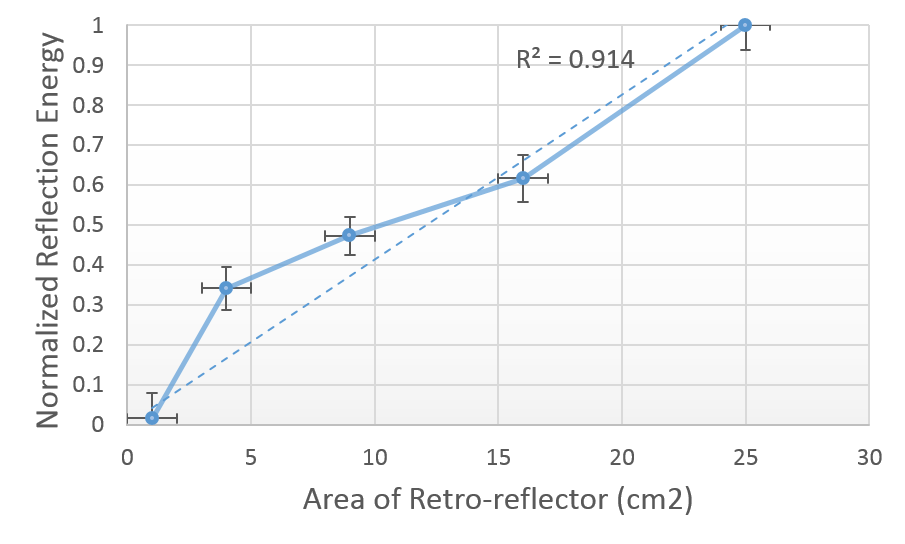
\includegraphics[width=0.46\columnwidth]{retro_size.png}\label{fig:retro2}
	  }
%      \vspace{-1em}
      \caption{Energy concentrating property of a retro-reflector when the light source emits omni-directional lights and the relationship between reflected energy and the retro-reflector size. }\label{fig:retro}
  \end{center}
%  \vspace{-0.3in}
\end{figure}


\paragraph{Liquid Crystal Display (LCD)}
In terms of embedding information bits on the reflected light, special retro-reflector can alter the amplitude by electronically controlling the reflection or absorption using for example MEMS technologies \cite{expensive,expensive2}. In our case, we hope to use ordinary, off-the-shelf retro-reflector fabrics. In order to modulate the lights reflected by such fabric, we resort to a liquid crystal display that can pass or block light under the control of electrical field. 


\begin{figure}[th]
  \begin{center}
      \subfigure[LCD Principle \cite{eavesdrop2}]{
        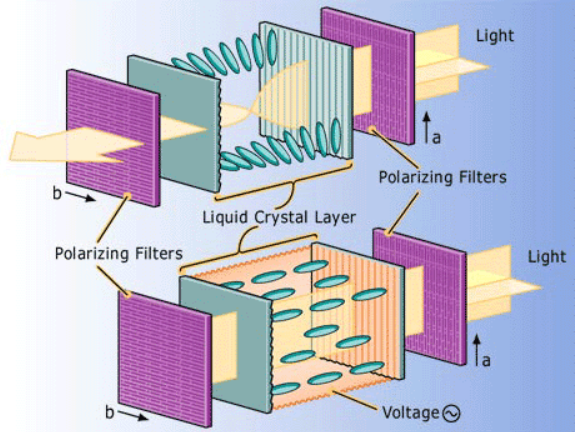
\includegraphics[width=0.48\columnwidth]{lcdworks-crop.png}\label{fig:lcdworks}
      } 
      \hfill
      \subfigure[LCD Driver]{
        \includegraphics[width=0.46\columnwidth]{../illustrations/conventional_LCD_driver.eps}\label{fig:lcd-circuits}
	  }
%      \vspace{-1em}
      \caption{The structure and principle of LCD, and its typical driving circuits. }\label{fig:lcd}
  \end{center}
%  \vspace{-0.3in}
\end{figure}

An LCD is a multi-layer sandwich structure. At the two far ends of the LCD panel are two polarizer films. The two polarizers can be parallel or perpendicular to each other. In the middle are two glass electrodes that encompassing a layer of the nematic phase liquid crystals, as shown in \figref{fig:lcdworks}. 
An LCD works as follows: when the incoming light passes through the first polarizer, it becomes polarized. Depending on the actual liquid crystal state, the polarity of the light will be changed or remain unchanged. 
In the natural state of the liquid crystal, its molecules are twisted. It will change the polarity of the light passing through it. If an electric field is imposed (by the two surrounding glass electrodes) on the liquid crystal, its molecules will become untwisted. The polarity of the light will not be affected when passing through. The light will finally be passed or blocked by the second polarizer on the other end, depending the conformance of their polarity \cite{eavesdrop2}. %http://qxwujoey.tripod.com/lcd.htm} 
%The reason we see the coloured images are due to the colour filter, light passes through the filtered cells creates the colors. There is also a colour filter containing the 3 primary colours (red, green and blue). 
At a high level, the polarization changes as the voltage added on it. At a low voltage, the incoming light traverses the LCD to hit the retro-reflector, and reflected light also traverses the LCD; At a high voltage, the incoming light is rejected by the LCD. 


%\p{Charging and discharging circuitry, as we will use them in the energy reuse. }
%The LCD usually consumes a little amount of current, but requires a relatively high voltage. For example, the LCD we used would start to take effect at 2.0V, and the desired working voltage is as high as 10V. In practice, we found a voltage of 6.0V will work. \todo{Explain the circuits, especially the charging/discharging paths.} We notice that the LCD itself is capacitor. \todo{need to further explain it's consequence. Postpone to the energy reuse section.}


%However, one disadvantage of LCDs are their low refresh rate, e.g., 60 or 75 Hz, which is too low for data communication. Fortunately, we find \textit{LCD shutters} with much higher refresh rate (up to 1KHz \hl{cite}). Fig.~\ref{fig:retrolcd} shows the basic principle of a retro-reflector with an LCD coverage.
